\section{Bluetooth}
\subsection{Présentation}
\begin{frame}
	\begin{minipage}[t]{0.25\linewidth}
		\uncover<2->{
			\begin{figure}
				\includegraphics[height=2.5cm]{img/bt_logo.png}
				\caption{Logo Bluetooth}
			\end{figure}
		}
	\end{minipage}\hfill
	\begin{minipage}[t]{0.72\linewidth}
		{ \footnotesize
		\uncover<1->{
			\begin{block}{Historique}
				\begin{itemize}
					\item 1994 : Création ( Ericsson )
					\item 1998 : SIG (Ericsson, Intel, Nokia, Toshiba)
					\item 1999 : v1.0
					\item 2004 : v2.0 : Basic Rate / Enhanced Data Rate
					\item 2010 : v4.0 Low Energy
					\item 2014 : v4.2
				\end{itemize}
			\end{block}
		}
		\uncover<3->{
			\begin{block}{Caractéristiques physiques}
				\begin{itemize}
					\item 2.4 GHz
					\item Max 24Mb/s
					\item 79 cannaux, AFH
					\item Conso : 1W
				\end{itemize}
			\end{block}
		}
	}
	\end{minipage}
\end{frame}

% Présenter des schémas
\subsection{Architecture logique}

\begin{frame}
	\begin{minipage}[t]{0.45\linewidth}
	\uncover<1->{
		\begin{figure}
			\vspace{0.5cm}
			\includegraphics[height=5.5cm]{img/arch_core.png}
			\caption{Bluetooth core}
		\end{figure}
	}
	\end{minipage}
	\begin{minipage}[t]{0.52\linewidth}
		{ \footnotesize
		\uncover<2->{
		\begin{block}{Host}
			\begin{itemize}
				\item Logique Métier
				\item Scheduling
				\item Buffering
			\end{itemize}
		\end{block}
		}
		\uncover<3->{
		\begin{block}{Host to Controller}
			\begin{itemize}
				\item Host to Controller Interface
				\item Sychronous Connection-Oriented
				\item Asychronous Connection-Less
			\end{itemize}
		\end{block}
	}
		\uncover<4->{
		\begin{block}{Controller}
			\begin{itemize}
				\item Connexion
				\item Découverte
			\end{itemize}
		\end{block}
		}
	}
	\end{minipage}
\end{frame}

\begin{frame}
\begin{minipage}[t]{0.60\linewidth}
	\begin{figure}
		\includegraphics[height=5.5cm]{img/arch_log_hci.png}
		\caption{Host to Controller Interface}
	\end{figure}
\end{minipage}
\begin{minipage}[t]{0.30\linewidth}
	\begin{block}{HCI}
		\begin{itemize}
			\item Uniformisation
			\item Abstraction
		\end{itemize}
		Commandes : 
		\begin{itemize}
			\item Données
			\item Configuration
			\item Évènements
		\end{itemize}
	\end{block}
\end{minipage}
\end{frame}

\begin{frame}
	\begin{minipage}[t]{0.60\linewidth}
		\begin{figure}
			\includegraphics[height=5cm]{img/arch_log_l2cap.png}
			\caption{Logical Link Control and Adaptation Protocol}
		\end{figure}
	\end{minipage}
	\begin{minipage}[t]{0.30\linewidth}
		\begin{block}{L2CAP}
			Socle pour de nombreux profils :
			\begin{itemize}
				\item Multiplexage
				\item Buffering
				\item QoS
				\item Scheduling
			\end{itemize}
		\end{block}
	\end{minipage}
\end{frame}

\begin{frame}
	\begin{minipage}[t]{0.60\linewidth}
		\uncover<1->{
		\begin{figure}
			\includegraphics[height=5cm]{img/arch_log_all.png}
			\caption{Profils}
		\end{figure}
		}
	\end{minipage}
	\begin{minipage}[t]{0.38\linewidth}
		\uncover<2->{
		\begin{block}{Protocoles}
			\begin{itemize}
				\item RFCOMM
				\item BNEP
				\item AVCTP { \tiny( controle A/V )}
				\item AVDTP { \tiny ( transport  A/V )}
			\end{itemize}
		\end{block}
		}
		\uncover<3->{
		\begin{block}{Profils}
			{ \footnotesize
			\begin{itemize}
				\item Serial Port Profile
				\item Human Interface Device
				\item Personnal Area Network
				\item Phone Book Access Profile
			\end{itemize}
			}
		\end{block}
		}
	\end{minipage}
\end{frame}

\subsection{Appairage}
\begin{frame}
	\begin{minipage}[t]{0.45\linewidth}
		\uncover<1->{
		\begin{block}{Découverte}
			\begin{enumerate}
				\item Inquiry
				\item Paging
				\item Connexion
			\end{enumerate}
		\end{block}
		}
		\uncover<2->{
		\begin{block}{Appairage}
			\begin{itemize}
				\item Connexion automatique,
				\item sécurisée,
				\item authentifiée,
				\item adaptée à l'appareil.
			\end{itemize}
		\end{block}
		}
	\end{minipage}
	\begin{minipage}[t]{0.45\linewidth}
		\uncover<3->{
		\begin{figure}
		\includegraphics[height=2cm]{img/nex_5.png}
		\end{figure}
		}
		\uncover<4->{
		\begin{figure}
		\includegraphics[height=1.5cm]{img/headset.png}
		\end{figure}
		}
		\uncover<5->{
		\begin{figure}
		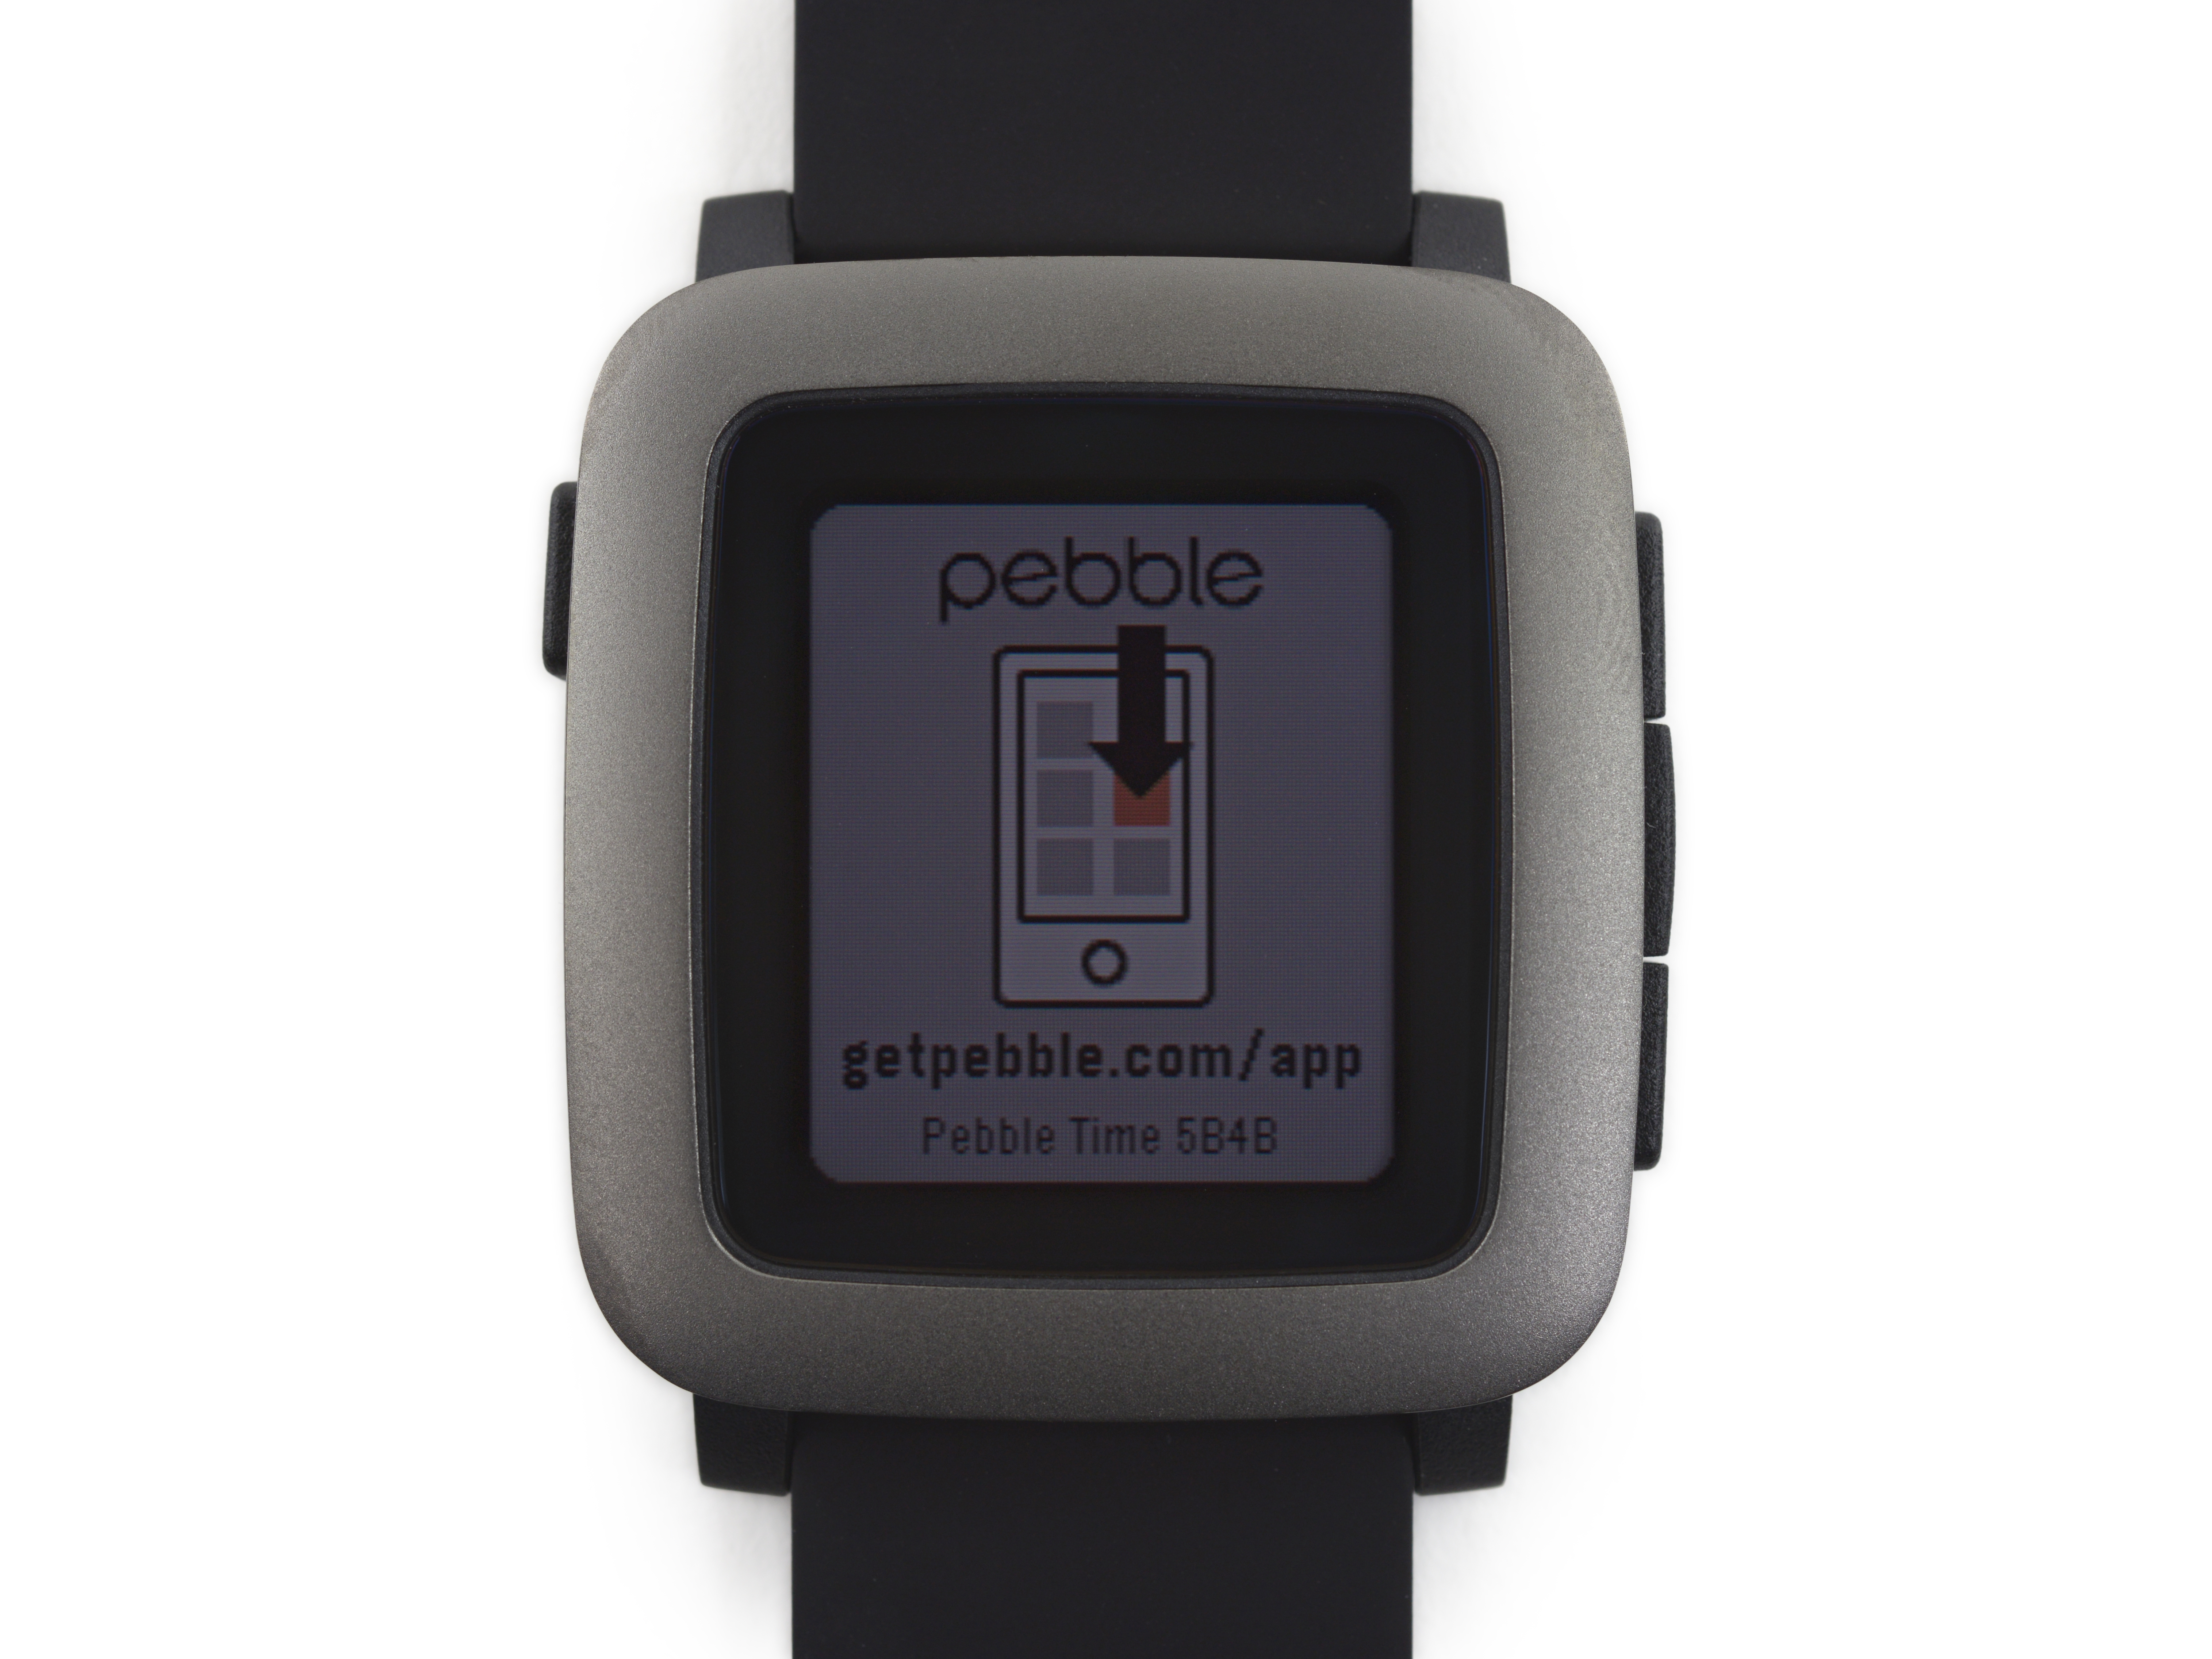
\includegraphics[height=1.5cm]{img/pt.jpg}
		\end{figure}
		}
	\end{minipage}
\end{frame}

\subsection{Découverte de services}
\begin{frame}
\begin{minipage}[t]{0.70\linewidth}

\begin{figure}
\includegraphics[height=5.5cm]{img/sdp.png}
\caption{Service Discovery Protocol}
\end{figure}


\end{minipage}
\begin{minipage}[t]{0.27\linewidth}
\begin{block}{UUID}
Identifient des :
\begin{itemize}
\item Profils
\item Protocoles
\item Attributs GATT
\end{itemize}
\end{block}

\end{minipage}
{\tiny Liste : https://www.bluetooth.com/specifications/assigned-numbers/service-discovery}
\end{frame}
